\documentclass[11pt,]{article}
\usepackage[left=1in,top=1in,right=1in,bottom=1in]{geometry}
\newcommand*{\authorfont}{\fontfamily{phv}\selectfont}
  \usepackage[]{mathpazo}
  
  
  \usepackage[T1]{fontenc}
\usepackage[utf8]{inputenc}



\usepackage{abstract}
\renewcommand{\abstractname}{}    % clear the title
\renewcommand{\absnamepos}{empty} % originally center

\renewenvironment{abstract}
{{%
  \setlength{\leftmargin}{0mm}
  \setlength{\rightmargin}{\leftmargin}%
}%
  \relax}
{\endlist}

\makeatletter
\def\@maketitle{%
  \newpage
  %  \null
  %  \vskip 2em%
    %  \begin{center}%
    \let \footnote \thanks
  {\fontsize{18}{20}\selectfont\raggedright  \setlength{\parindent}{0pt} \@title \par}%
}
%\fi
\makeatother


  
  
  \setcounter{secnumdepth}{0}

      \usepackage{color}
  \usepackage{fancyvrb}
  \newcommand{\VerbBar}{|}
  \newcommand{\VERB}{\Verb[commandchars=\\\{\}]}
  \DefineVerbatimEnvironment{Highlighting}{Verbatim}{commandchars=\\\{\}}
  % Add ',fontsize=\small' for more characters per line
  \usepackage{framed}
  \definecolor{shadecolor}{RGB}{248,248,248}
  \newenvironment{Shaded}{\begin{snugshade}}{\end{snugshade}}
  \newcommand{\AlertTok}[1]{\textcolor[rgb]{0.94,0.16,0.16}{#1}}
  \newcommand{\AnnotationTok}[1]{\textcolor[rgb]{0.56,0.35,0.01}{\textbf{\textit{#1}}}}
  \newcommand{\AttributeTok}[1]{\textcolor[rgb]{0.77,0.63,0.00}{#1}}
  \newcommand{\BaseNTok}[1]{\textcolor[rgb]{0.00,0.00,0.81}{#1}}
  \newcommand{\BuiltInTok}[1]{#1}
  \newcommand{\CharTok}[1]{\textcolor[rgb]{0.31,0.60,0.02}{#1}}
  \newcommand{\CommentTok}[1]{\textcolor[rgb]{0.56,0.35,0.01}{\textit{#1}}}
  \newcommand{\CommentVarTok}[1]{\textcolor[rgb]{0.56,0.35,0.01}{\textbf{\textit{#1}}}}
  \newcommand{\ConstantTok}[1]{\textcolor[rgb]{0.00,0.00,0.00}{#1}}
  \newcommand{\ControlFlowTok}[1]{\textcolor[rgb]{0.13,0.29,0.53}{\textbf{#1}}}
  \newcommand{\DataTypeTok}[1]{\textcolor[rgb]{0.13,0.29,0.53}{#1}}
  \newcommand{\DecValTok}[1]{\textcolor[rgb]{0.00,0.00,0.81}{#1}}
  \newcommand{\DocumentationTok}[1]{\textcolor[rgb]{0.56,0.35,0.01}{\textbf{\textit{#1}}}}
  \newcommand{\ErrorTok}[1]{\textcolor[rgb]{0.64,0.00,0.00}{\textbf{#1}}}
  \newcommand{\ExtensionTok}[1]{#1}
  \newcommand{\FloatTok}[1]{\textcolor[rgb]{0.00,0.00,0.81}{#1}}
  \newcommand{\FunctionTok}[1]{\textcolor[rgb]{0.00,0.00,0.00}{#1}}
  \newcommand{\ImportTok}[1]{#1}
  \newcommand{\InformationTok}[1]{\textcolor[rgb]{0.56,0.35,0.01}{\textbf{\textit{#1}}}}
  \newcommand{\KeywordTok}[1]{\textcolor[rgb]{0.13,0.29,0.53}{\textbf{#1}}}
  \newcommand{\NormalTok}[1]{#1}
  \newcommand{\OperatorTok}[1]{\textcolor[rgb]{0.81,0.36,0.00}{\textbf{#1}}}
  \newcommand{\OtherTok}[1]{\textcolor[rgb]{0.56,0.35,0.01}{#1}}
  \newcommand{\PreprocessorTok}[1]{\textcolor[rgb]{0.56,0.35,0.01}{\textit{#1}}}
  \newcommand{\RegionMarkerTok}[1]{#1}
  \newcommand{\SpecialCharTok}[1]{\textcolor[rgb]{0.00,0.00,0.00}{#1}}
  \newcommand{\SpecialStringTok}[1]{\textcolor[rgb]{0.31,0.60,0.02}{#1}}
  \newcommand{\StringTok}[1]{\textcolor[rgb]{0.31,0.60,0.02}{#1}}
  \newcommand{\VariableTok}[1]{\textcolor[rgb]{0.00,0.00,0.00}{#1}}
  \newcommand{\VerbatimStringTok}[1]{\textcolor[rgb]{0.31,0.60,0.02}{#1}}
  \newcommand{\WarningTok}[1]{\textcolor[rgb]{0.56,0.35,0.01}{\textbf{\textit{#1}}}}
        
    \usepackage{graphicx,grffile}
\makeatletter
\def\maxwidth{\ifdim\Gin@nat@width>\linewidth\linewidth\else\Gin@nat@width\fi}
\def\maxheight{\ifdim\Gin@nat@height>\textheight\textheight\else\Gin@nat@height\fi}
\makeatother
% Scale images if necessary, so that they will not overflow the page
% margins by default, and it is still possible to overwrite the defaults
% using explicit options in \includegraphics[width, height, ...]{}
\setkeys{Gin}{width=\maxwidth,height=\maxheight,keepaspectratio}
  
    \title{Homework 1  }
  
  
  
  \author{\Large \vspace{0.05in} \newline\normalsize\emph{}  }
  
  
  \date{}

\usepackage{titlesec}

\titleformat*{\section}{\normalsize\bfseries}
\titleformat*{\subsection}{\normalsize\itshape}
\titleformat*{\subsubsection}{\normalsize\itshape}
\titleformat*{\paragraph}{\normalsize\itshape}
\titleformat*{\subparagraph}{\normalsize\itshape}


  
      
  
  \newtheorem{hypothesis}{Hypothesis}
\usepackage{setspace}

\makeatletter
\@ifpackageloaded{hyperref}{}{%
  \ifxetex
  \PassOptionsToPackage{hyphens}{url}\usepackage[setpagesize=false, % page size defined by xetex
                                                 unicode=false, % unicode breaks when used with xetex
                                                 xetex]{hyperref}
  \else
    \PassOptionsToPackage{hyphens}{url}\usepackage[unicode=true]{hyperref}
  \fi
}

\@ifpackageloaded{color}{
  \PassOptionsToPackage{usenames,dvipsnames}{color}
}{%
  \usepackage[usenames,dvipsnames]{color}
}
\makeatother
\hypersetup{breaklinks=true,
bookmarks=true,
pdfauthor={ ()},
pdfkeywords = {},  
pdftitle={Homework 1},
colorlinks=true,
citecolor=blue,
urlcolor=blue,
linkcolor=magenta,
pdfborder={0 0 0}}
\urlstyle{same}  % don't use monospace font for urls

% set default figure placement to htbp
\makeatletter
\def\fps@figure{htbp}
\makeatother

\setlength{\abovedisplayskip}{.2pt}
\setlength{\belowdisplayskip}{.2pt}
\usepackage{placeins}
\usepackage{setspace}
\usepackage{chngcntr}
\usepackage{multicol}
\usepackage{lscape}
\counterwithin{figure}{section}
\counterwithin{table}{section}
\usepackage{mathrsfs}
\usepackage{mathtools}
\usepackage{multirow}
\newtheorem{theorem}{Theorem}
\usepackage[linesnumbered,algoruled,boxed,lined,commentsnumbered]{algorithm2e}
\usepackage{bm}
\usepackage{framed}
\usepackage{xcolor}
\colorlet{shadecolor}{orange!15}


% add tightlist ----------
\providecommand{\tightlist}{%
\setlength{\itemsep}{0pt}\setlength{\parskip}{0pt}}

\begin{document}

% \pagenumbering{arabic}% resets `page` counter to 1 
%
% \maketitle

{% \usefont{T1}{pnc}{m}{n}
\setlength{\parindent}{0pt}
\thispagestyle{plain}
{\fontsize{18}{20}\selectfont\raggedright 
\maketitle  % title \par  

}

{
  \vskip 13.5pt\relax \normalsize\fontsize{11}{12} 
  \textbf{\authorfont } \hskip 15pt \emph{\small }   
  
}

}






\vskip 6.5pt


\noindent  1.1

Download the daily, weekly and monthly prices for the Nasdaq index and
the IBM stock from Yahoo. Reproduce figures 1.3-8 using the Nasdaq index
and the IBM stock data. For 1.1, using the data from Jan 1985 - Aug
2018.

\begin{Shaded}
\begin{Highlighting}[]
\CommentTok{# Download the data}
\KeywordTok{library}\NormalTok{(quantmod)}
\CommentTok{# start <- as.Date("1985-01-01")}
\CommentTok{# end <- as.Date("2018-08-29")}
\CommentTok{# getSymbols("^IXIC", src = "yahoo", from = start, to = end)}
\CommentTok{# getSymbols("IBM", src = "yahoo", from = start, to = end)}
\CommentTok{# save to avoid reloading }
\CommentTok{# saveRDS(IXIC, "~/workspace/st790-financial-stats/data/ixic.rds")}
\CommentTok{# saveRDS(IBM, "~/workspace/st790-financial-stats/data/ibm.rds")}
\end{Highlighting}
\end{Shaded}

For NASDAQ:

\begin{Shaded}
\begin{Highlighting}[]
\CommentTok{# Read in data }
\NormalTok{IXIC <-}\StringTok{ }\KeywordTok{readRDS}\NormalTok{(}\StringTok{"~/workspace/st790-financial-stats/data/ixic.rds"}\NormalTok{)}
\NormalTok{IBM <-}\StringTok{ }\KeywordTok{readRDS}\NormalTok{(}\StringTok{"~/workspace/st790-financial-stats/data/ibm.rds"}\NormalTok{)}
\CommentTok{# Extract}
\NormalTok{daily <-}\StringTok{ }\KeywordTok{log}\NormalTok{(}\KeywordTok{dailyReturn}\NormalTok{(IXIC)}\OperatorTok{+}\DecValTok{1}\NormalTok{)}
\NormalTok{weekly <-}\StringTok{ }\KeywordTok{log}\NormalTok{(}\KeywordTok{weeklyReturn}\NormalTok{(IXIC)}\OperatorTok{+}\DecValTok{1}\NormalTok{)}
\NormalTok{monthly <-}\StringTok{ }\KeywordTok{log}\NormalTok{(}\KeywordTok{monthlyReturn}\NormalTok{(IXIC)}\OperatorTok{+}\DecValTok{1}\NormalTok{)}
\CommentTok{# Plot }
\KeywordTok{par}\NormalTok{(}\DataTypeTok{mar=}\KeywordTok{c}\NormalTok{(}\DecValTok{1}\NormalTok{,}\DecValTok{3}\NormalTok{,}\DecValTok{2}\NormalTok{,}\DecValTok{1}\NormalTok{),}\DataTypeTok{mfrow=}\KeywordTok{c}\NormalTok{(}\DecValTok{4}\NormalTok{,}\DecValTok{1}\NormalTok{)) }
\KeywordTok{plot}\NormalTok{(}\KeywordTok{index}\NormalTok{(IXIC), }\KeywordTok{as.numeric}\NormalTok{(IXIC}\OperatorTok{$}\NormalTok{IXIC.Close), }\DataTypeTok{type =} \StringTok{"l"}\NormalTok{, }
     \DataTypeTok{ylab =} \StringTok{"daily price"}\NormalTok{)}
\KeywordTok{plot}\NormalTok{(}\KeywordTok{index}\NormalTok{(daily), daily, }\DataTypeTok{type =} \StringTok{"l"}\NormalTok{, }
     \DataTypeTok{ylab=}\StringTok{"daily log return"}\NormalTok{)}
\KeywordTok{plot}\NormalTok{(}\KeywordTok{index}\NormalTok{(weekly), weekly, }\DataTypeTok{type =} \StringTok{"l"}\NormalTok{,}
     \DataTypeTok{ylab=}\StringTok{"weekly log return"}\NormalTok{)}
\KeywordTok{plot}\NormalTok{(}\KeywordTok{index}\NormalTok{(monthly), monthly, }\DataTypeTok{type =} \StringTok{"l"}\NormalTok{, }
     \DataTypeTok{ylab=}\StringTok{"monthly log return"}\NormalTok{)}
\end{Highlighting}
\end{Shaded}

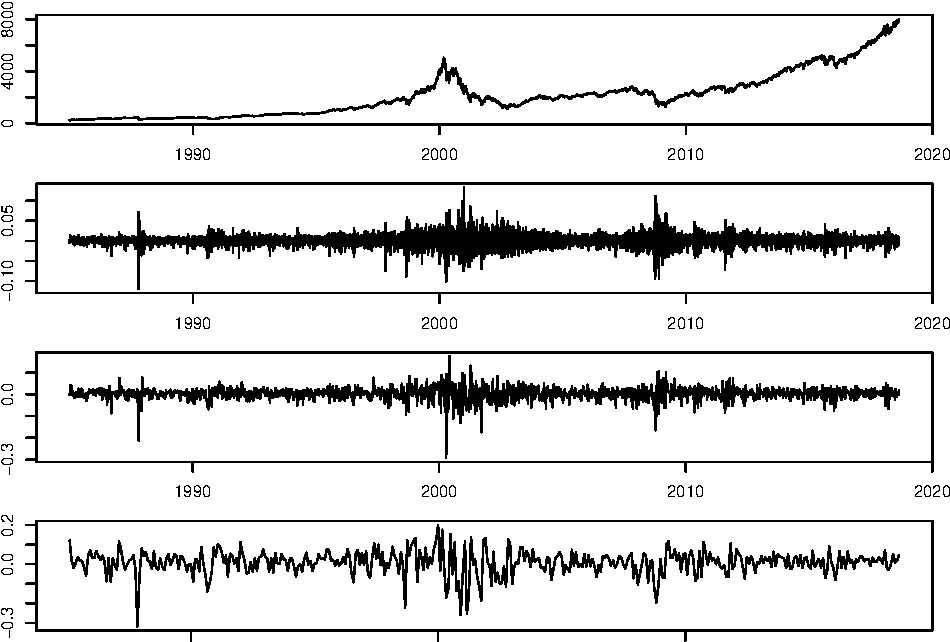
\includegraphics{hw1_files/figure-latex/unnamed-chunk-3-1.pdf}

For IBM:

\begin{Shaded}
\begin{Highlighting}[]
\CommentTok{# Extract}
\NormalTok{daily <-}\StringTok{ }\KeywordTok{log}\NormalTok{(}\KeywordTok{dailyReturn}\NormalTok{(IBM)}\OperatorTok{+}\DecValTok{1}\NormalTok{)}
\NormalTok{weekly <-}\StringTok{ }\KeywordTok{log}\NormalTok{(}\KeywordTok{weeklyReturn}\NormalTok{(IBM)}\OperatorTok{+}\DecValTok{1}\NormalTok{)}
\NormalTok{monthly <-}\StringTok{ }\KeywordTok{log}\NormalTok{(}\KeywordTok{monthlyReturn}\NormalTok{(IBM)}\OperatorTok{+}\DecValTok{1}\NormalTok{)}
\CommentTok{# Plot }
\KeywordTok{par}\NormalTok{(}\DataTypeTok{mar=}\KeywordTok{c}\NormalTok{(}\DecValTok{1}\NormalTok{,}\DecValTok{3}\NormalTok{,}\DecValTok{2}\NormalTok{,}\DecValTok{1}\NormalTok{),}\DataTypeTok{mfrow=}\KeywordTok{c}\NormalTok{(}\DecValTok{4}\NormalTok{,}\DecValTok{1}\NormalTok{)) }
\KeywordTok{plot}\NormalTok{(}\KeywordTok{index}\NormalTok{(IBM), }\KeywordTok{as.numeric}\NormalTok{(IBM}\OperatorTok{$}\NormalTok{IBM.Close), }\DataTypeTok{type =} \StringTok{"l"}\NormalTok{, }
     \DataTypeTok{ylab =} \StringTok{"daily price"}\NormalTok{)}
\KeywordTok{plot}\NormalTok{(}\KeywordTok{index}\NormalTok{(daily), daily, }\DataTypeTok{type =} \StringTok{"l"}\NormalTok{, }
     \DataTypeTok{ylab=}\StringTok{"daily log return"}\NormalTok{)}
\KeywordTok{plot}\NormalTok{(}\KeywordTok{index}\NormalTok{(weekly), weekly, }\DataTypeTok{type =} \StringTok{"l"}\NormalTok{,}
     \DataTypeTok{ylab=}\StringTok{"weekly log return"}\NormalTok{)}
\KeywordTok{plot}\NormalTok{(}\KeywordTok{index}\NormalTok{(monthly), monthly, }\DataTypeTok{type =} \StringTok{"l"}\NormalTok{, }
     \DataTypeTok{ylab=}\StringTok{"monthly log return"}\NormalTok{)}
\end{Highlighting}
\end{Shaded}

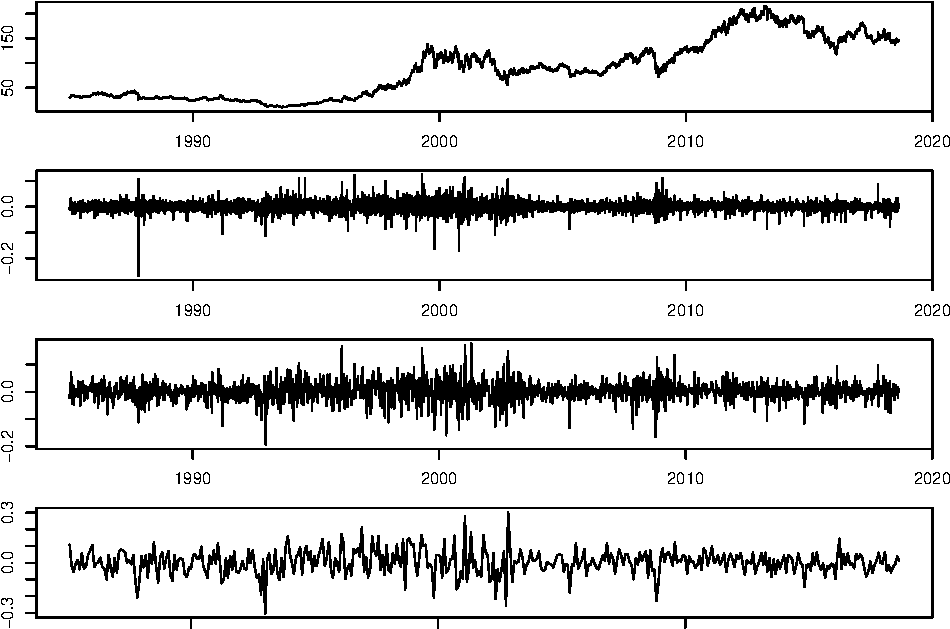
\includegraphics{hw1_files/figure-latex/unnamed-chunk-4-1.pdf}

1.3 Consider the following quote from Eugene Fama who was Myron Scholes'
thesis adviser: ``If the population of prices changes is strictly
normal, on the average for any stock\ldots{} an observation more than 5
standard deviations from the mean should be observed once every 7000
years. In fact such observations seem to occur about once every 3 or 5
years.'' For
\(X \sim N(\mu, \sigma^2), P(|X-\mu| > 5\sigma) = 5.733 \times 10^{-7}\),
deduce how many observations per year Fama was implicitly assumining to
be made. If a year is defined as 252 trading days and daily returns are
normal, how many years is it expected to take to get a 5 standard
deviation event? How does this answwer to the last question change when
the daily returns follow the t-distribution with 4 degrees of freedom?

1.8 According to the efficient market hypothesis, is the return of a
portfolio predictable? Is the volatility of a portfolio predictable?
State the most appropriate mathematical form of the efficient market
hypothesis.

1.9 If the Ljung-Box test is employed to test the efficient market
hypothesis, what null hypothesis is to be tested? If the autocorrelation
for the first 4 lags of the montly log-returns of the S\&P500 is:

\[
\hat{\rho}(1) = .2, \quad \hat{\rho}(2) = -0.15, \quad \hat{\rho}(3) = 0.25, \quad \hat{\rho}(4) = 0.12
\] based on the last 5 years of data, is the efficient market hypothesis
reasonable?

1.13 Let \(S_t\) be the price of an asset at time \(t\). One version of
the EMH assumes that the prices of any asset form a martingale process
in the sense that:

\[
E(S_{t+1}|S_t, S_{t-1}, \ldots ) = S_t \quad \forall t
\]

To understand the implication of this assumption, we consider the
following simple investment strategy. With initial capital \(C_0\)
dollars, at the time \(t\) we hold \(\alpha_t\) dollars in cash and
\(\beta_t\) shares of an asset at the price \(S_t\). Hence the value of
our investment at time \(t\) is \(C_t=\alpha_t + \beta_t S_t\). Suppose
that our investment is self-financing in the sense that

\[
C_{t+1} = \alpha_t + \beta_t S_{t+1} = \alpha_{t+1} + \beta_{t+1} S_{t+1}
\]

and our investment strategy is entirely determined by the asset prices
up to the time \(t\). Show that if \(S_t\) is a martingale process,
there exist no strategies such that \(C_{t+1} > C_t\) with probability
1.
\newpage
\singlespacing 
\end{document}
